 
\documentclass{beamer}
\setbeamertemplate{section in toc}[sections numbered]
\usefonttheme[onlymath]{serif}
\beamertemplatenavigationsymbolsempty
\setbeamertemplate{footline}{% 
  \hfill% 
  \usebeamercolor[gray!50]{page number in head/foot}% 
  \usebeamerfont{page number in head/foot}% 
  \insertframenumber\,/\,\inserttotalframenumber%
}
\usepackage{amsmath}
\usepackage{graphicx}
% \usepackage{caption}
% \usepackage[skip=0pt]{subcaption}
% \usepackage[tight,FIGTOPCAP]{subfigure}
\usepackage{lmodern}
\usepackage[round]{natbib}
\usepackage{braket}
\usepackage{color}
\usepackage{bm}
\usepackage{amssymb}
\usepackage{bbold}
\usepackage{tikz}
\usepackage{empheq}
\usepackage{stackengine}
\usepackage{framed}
\usepackage[percent]{overpic}
\usepackage{adjustbox}
\DeclareMathOperator{\sgn}{sgn}
\tikzset{>=latex}
\newcommand{\blue}[1]{{\color{blue}{#1}}}
\newcommand{\md}{\mathrm{d}}
\newcommand{\ms}{\mathsf}
\newcommand{\bs}{\boldsymbol}
\newcommand{\mc}{\mathcal}
\renewcommand{\(}{\left(}
\renewcommand{\)}{\right)}
\renewcommand{\[}{\left[}
\renewcommand{\]}{\right]}

%Information to be included in the title page:
\title{Toric Code}
%\author{Apoorv Tiwar, Ammar Jahin, and Yuxuan Wang}
%\institute{University of Florida}
\date{University of Florida, \today}

\begin{document}
\frame{\titlepage} 
\AtBeginSection[]
{
\begin{frame}
    \frametitle{Outline}
    \tableofcontents[currentsection]
\end{frame}
}

\begin{frame}
    \frametitle{Two approaches to Kitaev toric code \citep{Kitaev_2003}}

    \begin{columns}
        \begin{column}{0.5\textwidth}
            \begin{center}
            As a discrete gauge theory
            \end{center}
        \end{column}
        \begin{column}{0.5\textwidth}
            \begin{center}
            As a quantum code
            \end{center}
        \end{column}
    \end{columns}

    \begin{columns}
        \begin{column}{0.5\textwidth}
            \begin{itemize}
                \item It's a $\mathbb{Z}_2$ gauge theory
                \item It has anyonic excitations
                \item Long range entanglement and topological order
            \end{itemize}
        \end{column}
        \begin{column}{0.5\textwidth}
            \begin{itemize}
                \item It implements a specific type of quantum code
                \item Allow error detection and error correction
                \item Allows for a restricted qubit operations
            \end{itemize}
        \end{column}
    \end{columns}
    \vspace{10pt}
    \pause
    \begin{center}
        \begin{framed}
            This talk will focus on the quantum code aspect. 
            \end{framed}
    \end{center}
\end{frame}
\begin{frame}
    \frametitle{Outline}

    \tableofcontents

\end{frame}
\section{Introduction: Noise reduction}
\subsection{Classical analog}
\begin{frame}
    \frametitle{The classical analog of the problem}
    Communication over a noisy channel,
    \begin{itemize}
        \item We have a string of $k$ bits that we want to \emph{send} over a noisy channel. 
        \item Each bit has a probability, $p_f$, to flip its value as it go through the channel. Errors can happen when sending data.
        \item How can we make this communication reliable? 
    \end{itemize}
    \pause
    Solutions: 
    \begin{enumerate}
        \item Physically build a more reliable channel. (Not always possible)
        \item Add redundancy to the sent signal, such that when errors happen we would still have a way of retrieving the original information (the original string of bits).
    \end{enumerate}

\end{frame}
\begin{frame}
    \frametitle{Classical coding theory}
    \begin{center}
    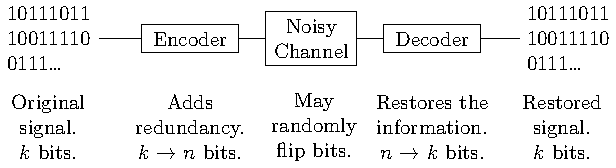
\includegraphics[scale=1]{classical_code_theory.pdf}
    \end{center}
    \pause
    Example: The repetition code. 
    \vspace{5pt}
    \begin{columns}
        \begin{column}{0.5\textwidth}
            \centering
            Encoder:
            
            $0 \rightarrow 000 $ 

            $1 \rightarrow 111 $ 

        \end{column}
        \begin{column}{0.5\textwidth}
            \centering
            Decoder (majority vote): 
            
            $\{000,001,010,100\} \rightarrow 0$ 

            $\{111,110,101,011\} \rightarrow 1 $ 
        \end{column}
    \end{columns}
    \vspace{10pt}
    If we had a probability $p_f$ of making an error (per bit) before, now we have a probability of $p_f^2$ of making an error. 
    \pause
    \begin{itemize}
        \item The repetition code is not efficient. 
        \item Other problems can be seen as a noisy channel problem. 
    \end{itemize}

\end{frame}
\begin{frame}
    \frametitle{The (quantum) problem}
    The same problem is amplified in the quantum world.
    A qubit is a two level quantum system, 
    \begin{align*}
        \ket{\psi} = c_0 \ket{0} + c_1 \ket{1}
    \end{align*}
    Suppose we have prepare a system of $k$ qubits in a specific state,
    \begin{align*}
        \ket{\Psi} = \bigotimes_{k}\ket{\psi_k}
    \end{align*} 
    \pause
    We want to preserve this state against information loss due to the effect of the environment (a noisy channel problem). 

    Same principle applies:
    \begin{itemize}
        \item Encode the $k$ qubit into a bigger space of $n$ qubits. 
    \end{itemize}
    \pause
    Difficulties with the quantum system: 
    \begin{itemize}
        \item A qubit cannot duplicated. $\ket{\Psi} \rightarrow \ket{\Psi} \otimes \ket{\Psi}$
        \item A measurement destroys the original state. 
        \item Errors are not just \emph{flips}.
    \end{itemize}
\end{frame}

\subsection{Quantum codes}
\begin{frame}
    \frametitle{Big picture of error correction}
    \begin{itemize}
        \item To correct an error, we first need to detect an error. 
        \item To detect an error, some sort of measurement must be done. (Measuring the error.) 
        \item Measuring the qubits themselves destroys all information. 
    \end{itemize}
    \pause
    A breakthrough came in 1995, \citep{Shor_1995}, to first entangle the system to ancillary qubits in such a way that measuring the ancillary qubits would measure the error. After which the appropriate correction can be done. 
    \pause
    Steps to error correction: 
    \begin{enumerate}
        \item Add redundancy, $k \rightarrow n$ qubits. A quantum code.
        \item Possible errors get introduced to the system. 
        \item Couple the system ancillary qubits.
        \item Measure the errors by measuring the ancillary qubits. Called a syndrome measurement. 
        \item Correct the error. 
    \end{enumerate}
\end{frame}


\begin{frame}
    \frametitle{Errors}

    \begin{enumerate}
        \item Coherent errors. They act as a unitary operator on the state. They don't entangle the qubits to the environment. \begin{align*}
            &\ket{\psi} \rightarrow E\ket{\psi} \\ 
            E &= \begin{bmatrix}
                E_{11} && E_{12} \\ 
                E_{21} && E_{22}
                \end{bmatrix}
        \end{align*}
        \pause
        \item Incoherent errors. They entangle the qubits to the environment. If $\ket{\Phi}$ represent the state of the environment, \begin{align*}
            \ket{\psi}\otimes\ket{\Phi} \rightarrow   D &\(\ket{\psi}\otimes\ket{\Phi}\) = a_{ij} E^i\ket{\psi}\otimes L^j\ket{\Phi} \\
            &D = a_{ij} E^i \otimes L^j
        \end{align*} 
    \end{enumerate}
    \pause
    Measuring the ancillary qubits destroys any entanglement between the qubits and the environment. For now we will focus on coherent errors. 
\end{frame}

\begin{frame}
    \frametitle{Coherent Errors}
    \begin{align*}
        E = \alpha_0 1 + \alpha_x X + \alpha_z Z + \alpha_{xy}  XZ
    \end{align*}
    There are unaccountably many errors that can occur to one qubit. 

    Part of Shor's breakthrough is that by measuring the error, one force the system into either an $X$-type error, or a $Z$-type error. 
    \begin{itemize}
        \item $X$ is a bit flip. 
        \item $Z$ is a \emph{phase} flip.
    \end{itemize}
    \pause
    \begin{framed}
        \centering
        Being able to measure $X$, and $Z$-type errors is enough to account for all errors. 
    \end{framed}
\end{frame}

\subsection{The three-qubit code}
\begin{frame}
    \frametitle{The three-qubit code}
    \framesubtitle{1. Adding redundancy}
    \begin{align*}
        \ket{\psi} = c_0 \ket{0} + c_1 \ket{1} \rightarrow \ket{\psi}_L= c_0 \ket{000} + c_1 \ket{111}
    \end{align*}
    \pause
    \begin{itemize}
        \item $\ket{\psi}_L \neq \ket{\psi} \otimes \ket{\psi} \otimes \ket{\psi}$.
        \item $\ket{000}$ is codeword for $\ket{0}$, $\ket{111}$ is codeword for $\ket{1}$.  
        \item The codeword space is a 2D subspace of the 8D logic state space,
    \end{itemize}
    \pause
    \begin{align*}
        &\mc C = \text{span}\{\ket{000}, \ket{111}\} \ \  \text{codeword subspace} \\ 
        &\mc F = \text{span}\{\ket{100}, \ket{011}, \ket{010}, \ket{101}, \ket{001}, \ket{110}\} \ \  \text{error subspace} \\ 
        &\mc H =\mc C \oplus \mc F \ \  \text{full Hilbert space}
    \end{align*}
    \pause
    \begin{itemize}
        \item $\{Z_1Z_2, Z_2Z_3\}$ are the (generators of) logic qubit stabilizers, 
    \end{itemize}
    \begin{align*}
        \{Z_1Z_2, Z_2Z_3\} \ket{\psi}_L = \ket{\psi}_L \ \ \text{for} \ket{\psi}_L \in \mc C
    \end{align*}
    Stabilizers can be used to define $\mc C$.
\end{frame}


\begin{frame}
    \frametitle{The three-qubit code}
    \framesubtitle{1. Adding redundancy}
    \begin{itemize}
        \item $(Z_1Z_2)^2 = 1$ and $(Z_2Z_3)^2 = 1$, both have eigenvalues of $\pm 1$.
        \item The stabilizers define four 2D orthonormal subspaces, the codeword space is one of them.  
    \end{itemize}
    \begin{table}
        \begin{tabular}{ |c c c| }
            \hline
                            & $Z_1Z_2= 1$ & $Z_1Z_2= -1$ \\ 
            $Z_2Z_3= 1$     & $\{\ket{000},\ket{111}\}$ &$\{\ket{100},\ket{011}\}$ \\ 
            $Z_2Z_3= -1$     & $\{\ket{001},\ket{110}\}$ &$\{\ket{010},\ket{101}\}$ \\
            \hline
        \end{tabular}
    \end{table}
    \pause
    For an error to be detected it needs to take the state \emph{out} of the codeword subspace. For $\ket{\psi}_L \in \mc C$,
    \begin{align*}
        \{X_1, X_2, X_3\} \ket{\psi}_L \in \mc F \\
        \{Z_1, Z_2, Z_3\} \ket{\psi}_L \in \mc C 
    \end{align*}
    The three-qubit code is very limited, it can only detect bit flips errors, and not phase flip errors.
\end{frame}

\begin{frame}
    \frametitle{The three-qubit code}
    \framesubtitle{2. Errors, and 3. Adding ancillary qubits}
    Errors:
    \begin{align*}
        &\ket{\psi}_L \rightarrow E_L\ket{\psi}_L \\
        &E_L = E_1E_2E_3 \\ 
        &E_{1,2,3} = \alpha_0 1 + \alpha_x X_{1,2,3} + \alpha_z Z_{1,2,3} + \alpha_{xz}  XZ_{1,2,3}
    \end{align*}
    \pause
    Adding ancillary qubits: 
    \begin{align*}
        E_L \ket{\psi}_L \rightarrow  & \ \ \ (1+Z_1Z_2)(1+Z_2 Z_3) E_L \ket{\psi}_L \otimes \ket{00} \\ 
        &+(1+Z_1Z_2)(1-Z_2 Z_3) E_L \ket{\psi}_L \otimes \ket{01} \\ 
        &+(1-Z_1Z_2)(1+Z_2 Z_3) E_L \ket{\psi}_L \otimes \ket{10} \\ 
        &+(1-Z_1Z_2)(1-Z_2 Z_3) E_L \ket{\psi}_L \otimes \ket{11} \\ 
    \end{align*}
    A syndrome measurement \emph{projects} the logical state into one of the four subspaces defined by the stabilizers, \citep{Shor_1995}.
\end{frame}
\begin{frame}
    \frametitle{Measuring the errors}
    \framesubtitle{4. Syndrome measurement, and 5. Making corrections}  

    To first order in $|\alpha_x|$, $|\alpha_z|$, $|\alpha_{xz}|$ (which we like to think they are not larger numbers as compared to 1): 
    \begin{table}
        \begin{tabular}{ |c c| }
            \hline
            Syndrome & Possible errors \\ 
            $00$ & $1, Z_1, Z_2, Z_3$ \\ 
            $01$ & $X_1$ \\
            $10$ & $X_3$ \\
            $11$ & $X_2$ \\
            \hline
        \end{tabular}
    \end{table}
    \pause
    \begin{itemize}
        \item As mentioned, it cannot detect phase flips. 
        \item For $X$-errors, we can detect which qubit had its value flipped, hence we can perform a unitary transformation that would undo the error. 
        \item Our communication over the noisy channel has improved assuming that errors act independently on each qubit.
        \item More elaborate code can detect $Z$-errors while being also more efficient. 
    \end{itemize}
\end{frame}
\section{Kitaev toric code}
\subsection{The model}
\begin{frame}
    \frametitle{Kitaev Toric Model}
    \begin{columns}
        \begin{column}{0.67\textwidth}
            \begin{itemize}
                \item A lattice model of spin-$1/2$ particles.
                \item Each unit cell has $2$ spin sites, $1$ and $2$.
                \item Local operators: $\{\vec{\sigma}_{1}(\bm R_i), \vec{\sigma}_{2}(\bm R_i)\}$
                \item Operators at different lattice sites commute.
            \end{itemize} 
        \end{column}
        \begin{column}{0.33\textwidth}
            \centering
            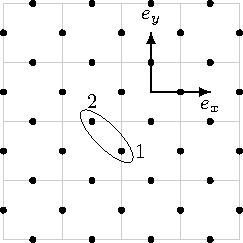
\includegraphics[scale=0.8]{spin_grid.pdf}
        \end{column}
    \end{columns}
    \pause
    \vspace{8pt}
    \begin{columns}
        \begin{column}{0.62\textwidth}
            The Hamiltonian: 
                \begin{align*}
                    H =& -\sum_{\bm R_i} \(A(\bm R_i)  + B(\bm R_i) \)\\
                    A(\bm R_i) = \ &\sigma^x_{2}(\bm R_i)\sigma^x_{1}(\bm R_i) \\  & \sigma^x_{2}  (\bm R_i + e_x)\sigma^x_{1} (\bm R_i+ e_y), \\
                    B(\bm R_i) = \ & \sigma^z_{1} (\bm R_i)\sigma^z_{2} (\bm R_i) \\ &\sigma^z_{1} (\bm R_i - e_x)\sigma^z_{2} (\bm R_i - e_y) 
                \end{align*}
        \end{column}
        \begin{column}{0.38\textwidth}
            \centering
            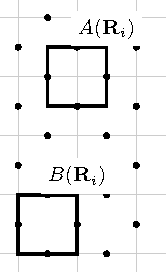
\includegraphics[scale = 1, trim=0 0 0 0, clip]{elementry_loops.pdf}

        \end{column}
    \end{columns}
\end{frame}

\begin{frame}
    \frametitle{Ground state of the Kitaev model}
    \begin{center}
        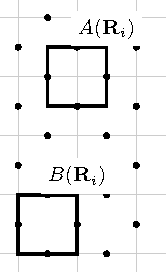
\includegraphics[scale = 1, trim=0 65 0 0,clip]{elementry_loops.pdf} \quad \quad 
        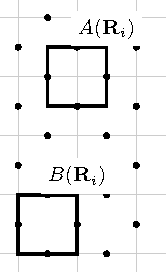
\includegraphics[scale = 1, trim=0 8 0 65,clip]{elementry_loops.pdf}
    \end{center}
    Notation: 
    
    $\sigma^x$: line perpendicular to unit cell edge at the spin site.

    $\sigma^z$: line along the unit cell edge at the spin site.
    \pause
    \begin{itemize}
        \item $A(\bm R_i)$ and $B(\bm R_i)$ are two different \emph{loops} in the system. 
        \item They only look like loops because of our choice of notation.
        \item No need for arrows on the loops.
        \item $A^2(\bm R_i) = 1$ and $B^2(\bm R_i) = 1$. Both have eigenvalues of $\pm 1$.
        \item $\[A(\bm R_i), B(\bm R_i)\] = 0$
    \end{itemize}
    \pause
    Ground sates $\ket{\Omega_0}$ of $H = -\sum_{\bm R_i} \(A(\bm R_i)  + B(\bm R_i) \)$ is defined by, 
    \begin{align*}
        A(\bm R_i)\ket{\Omega_0} = \ket{\Omega_0}, \  B(\bm R_i)\ket{\Omega_0} = \ket{\Omega_0}
    \end{align*}
\end{frame}


\subsection{The code}
\begin{frame}
    \frametitle{The code}
    We consider a $N \times N$ lattice on a torus. 
    \begin{itemize}
        \item The Hilbert space, $\mc H$, is $2^{2N^2}$ dimensional. 
        \item Codeword space, $\mc C$, is defined as \begin{align*}
            \mc C = \text{span}\{\ket{\Omega_0} \in \mc H : A(\bm R_i)\ket{\Omega_0} = \ket{\Omega_0}, \ B(\bm R_i)\ket{\Omega_0} = \ket{\Omega_0} \}
        \end{align*}
        \item This quantum code is called TOR($N$), the toric code.
        \item $A(\bm R_i)$, and $B(\bm R_i)$ are the code stabilizers. 
    \end{itemize}
    \pause
    \begin{columns}
        \begin{column}{0.8\textwidth}
            \begin{itemize}
                \item There are $2N^2 - 2$ independent stabilizers. There are $N^2$ $A(\bm R_i)$, and $N^2$ $B(\bm R_i)$ operators, but we have the following dependencies, \begin{align*}
                    \prod_{\bm R_i} A(\bm R_i) = 1, \prod_{\bm R_i} B(\bm R_i) = 1 \leftarrow  \text{No edges left.}
                \end{align*} 
                \item $\mc C$ is $(2^{2N^2})/(2^{2N^2-2}) = 2^2$ dimensional. It can encode 2 qubits. 
            \end{itemize}
        \end{column}
        \begin{column}{0.2\textwidth}
            \vspace{25pt}
            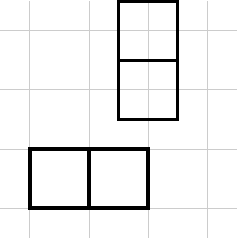
\includegraphics[scale = 0.6, trim=7 0 7 0,clip]{in_two_a_b.pdf}  
        \end{column}
    \end{columns}
\end{frame}
\begin{frame}
    \frametitle{What labels the ground states}
    Since the code stabilizers defines $2^{2N^2-2}$ 4D subspaces, we must label the $4$ states within each subspace by  other independent operators that commute with all the $A(\bm R_i)$ and $B(\bm R_i)$. 
    \pause
    \begin{columns}
        \begin{column}{0.55\textwidth}
            \begin{itemize}
                \item Every contractible loop can be decomposed into smaller loops of $A(\bm R_i)$ or $B(\bm R_i)$. 
                \item There are 4 different non-contractible loops. 
                \item $\{Z_1, Z_2, X_1, X_2\}$ commute with all contractible loops. 
                \item $\{Z_1, X_1\} = 0 $, $\{Z_2, X_2\} = 0 $
                \item The entire $2^{2N^2}$ Hilbert space can be labeled by the eigenvalues of, $\{Z_1, Z_1, A(\bm R_i), B(\bm R_i)\}$
            \end{itemize}
        \end{column}
        \begin{column}{0.45\textwidth}
            \vspace{10pt}
            \centering
            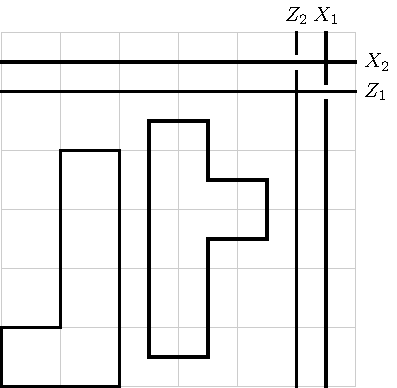
\includegraphics[scale=0.7, trim=0 0 0 0,clip]{decomp_loops.pdf}
        \end{column}
    \end{columns}
    
\end{frame}

\begin{frame}
    \frametitle{Errors}
    A general error can be any linear combination of,
    \begin{align*}
        E(\{\alpha^{l}_i, \beta^{m}_j\}) = \prod_{\substack{\bm R_i, \bm R_i\\ l, m}} (\sigma^x_l(\bm R_i))^{\alpha^{l}_i} (\sigma^z_m(\bm R_j))^{\beta^m_j},
    \end{align*}
    \pause
    % There are a total of $2^{2N^2+1}$. 
    These can be divided broadly into 3 categories: 
    \begin{enumerate}
        \item Contain only closed contractible loops. $E_1$.
        \item Contain one or more open strings. $E_2$.
        \item Contain one or more closed non-contractible loops. $E_3$.
    \end{enumerate}
    \pause
    \begin{itemize}
        \item Errors of type 1 are not errors at all, $E_1\ket{\Omega_0} = \ket{\Omega_0}$.
        \item Errors of type 2 can be detected by a syndrome measurement. 
        \item Errors of type 3 cannot be detected. 
    \end{itemize}
    \pause
    \begin{framed}
        Errors of type 3, must at least be $N$ long. And assuming errors act independently on each qubit, these errors would be exponentially suppressed, $e^{-\alpha N}$
    \end{framed}
\end{frame}
\begin{frame}
    \frametitle{Error detection, and correction}

    Open string operations anticommute with two stabilizer operators, one surrounding each end of the open ended loop.  
    \begin{columns}
        \begin{column}{0.5\textwidth}
            \begin{align*}
                B(\bm R_i) E_2 \ket{\Omega_0} = -E_2 \ket{\Omega_0}, \\ 
                \\
                A(\bm R_j) E_2 \ket{\Omega_0} = -E_2 \ket{\Omega_0}.
            \end{align*}
        \end{column}
        \begin{column}{0.5\textwidth}
            \centering
            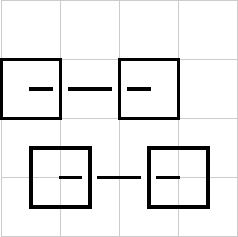
\includegraphics[scale=0.9]{open_closed_loop.pdf}
        \end{column}
    \end{columns}
    \pause
    \begin{itemize}
    \item These errors can be detected using a syndrome measurements. 
    \item Notice that $E_2\ket{\Omega_0}$ are excited states of the Hamiltonian, with $\Delta E \geqslant 2$. 
    \item Kitaev also suggested fixing these errors by coupling the system to a heat bath and cooling the system down. 
    \end{itemize}
    
\end{frame}

% \begin{frame}
%     \frametitle{Local perturbations}

%     It's important to check if the system is stable under local perturbations, otherwise the ground states might split and the system would lose the information encoded into its ground states.  
%     \begin{align*}
%         V =  - \sum_{\substack{\bm R_i, l}} \vec{h} \cdot \vec{\sigma}_{l}(\bm R_i) - \sum_{\substack{\bm R_i, \bm R_j \\ l, m }} \vec{\sigma}^{T}_{m}(\bm R_j) J^{m l}(\bm R_j, \bm R_i)\vec{\sigma}_{l} (\bm R_i)
%     \end{align*}

%     Splitting caused by this perturbation is $e^{-aN}$, for some finite $a$. 
% \end{frame}

\subsection{How to perform logical operations}

\begin{frame}
    \frametitle{Excitations of the toric code}
    Let's look at low energy excitations of the toric code. 
    \begin{itemize}
        \item We cannot have excitation with $\Delta E = 1$. This would violate 
        \begin{align*}
            \prod_{\bm R_i} A(\bm R_i) = 1, \ \ \prod_{\bm R_i} B(\bm R_i) = 1.
            \end{align*}\
        \item The lowest energy excitations have $\Delta E = 2$ and are obtained by applying string operators to the ground states. 
    \end{itemize}
    \pause
    \begin{center}
        \begin{columns}
            \begin{column}{0.5\textwidth}
                $S^x(t)\ket{\Omega_0},\  S^z(t)\ket{\Omega_0}$,
                which depend on
                \begin{enumerate}
                    \item The two end points
                    \item The homotopy of string connecting the two ends, how many non-contractible loops it make. Not the detailed path. 
                \end{enumerate}
            \end{column}
            \begin{column}{0.5\textwidth}
                \centering
                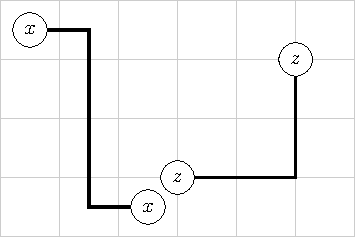
\includegraphics[scale = 0.8]{two_strings.pdf}
            \end{column}
        \end{columns}
    \end{center}
\end{frame}

\begin{frame}
    \frametitle{Allowed logic operaion using kitaev model}
    Remember, on a torus geometry, the ground state encode 2 qubits. We can do the following operation in the qubits:
    \begin{enumerate}
        \item $Z$ operation. 
        \begin{itemize}
            \item Create an a $z$-type particles pair. 
            \item Move one around one non-contractible loop. The direction determine which qubit get acted on. 
            \item Annihilate the two particles. 
        \end{itemize}
        \item $X$ operation. Using the same steps but with an $x$-type particle. 
    \end{enumerate}
    These operations do not give us a universal quantum computer. 
\end{frame}

\begin{frame}
    \frametitle{The dual lattice}

    For the same arrangement of spins there are two ways of defining the lattice. Both of them are equally valid. 
    \begin{columns}
        \begin{column}{0.55\textwidth}
            \begin{itemize}
                \item This highlights an important property of the system. 
            \end{itemize}
            Let $R_y(\theta)$ be the rotation operation around the $y$-axis then: 
            \begin{align*}
                R_y(90^\circ) A(\bm R_i) R^{-1}_y(90^\circ) = B^\prime(\bm R_i) \\
                R_y(90^\circ) B(\bm R_i) R^{-1}_y(90^\circ) = A^\prime(\bm R_i)
            \end{align*}
        \end{column}
        \begin{column}{0.45\textwidth}
            \begin{center}
            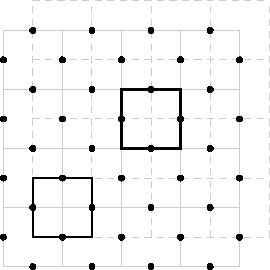
\includegraphics[scale=0.9]{dual_lattice.pdf}
            \end{center}
        \end{column}
    \end{columns}

    \begin{framed}
    This operation takes an $x$-type particle to a $z$-type particle. 
    \end{framed}

\end{frame}
\section{Anyonic nature of the excitations}
\begin{frame}
    \frametitle{The toric code in different geomtries}
    A (surprising) aspect about the toric code is that the ground state degeneracy depends on the genus, $g$, of the manifold. The toric code is $4^g$ degenerate. 
    
    \pause
    On a \emph{sphere} there are no non-contractible loops. $A(\bm R_i)$ and $B(\bm R_i)$ can label the entire Hilbert space. 
    \begin{columns}
        \begin{column}{0.5\textwidth}
            \begin{itemize}
                \item Hilbert space is $2^{12N^2}$ dimensional.
                \item $6N^2 \ B(\bm R_i)$ operators.
                \item $6N^2 + 2 \ A(\bm R_i)$ operators.
            \end{itemize}
        \end{column}
        \begin{column}{0.5\textwidth}
            \centering
            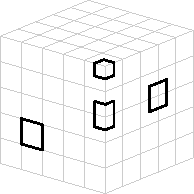
\includegraphics[scale=1.1]{toric_on_sphere.pdf}
        \end{column}
    \end{columns}
    \pause
    \begin{framed}
        The dependance of the ground state degeneracy on the geometry of the manifold is one of the defining features of topological order. 
    \end{framed}
\end{frame}
\begin{frame}
    \frametitle{Particle content of the toric code}

    \begin{itemize}
        \item No particles, 1.
        \item An $z$-type particle is referred to as electric charge, $e$.
        \item A $x$-type particle is referred to as a magnetic vortex, $m$.
        \item A combinations of an $e$ and an $m$ particle, $\psi = e \times m$
    \end{itemize}
    \pause
    Next we ask what is the statistics of these particles. 
    \begin{columns}
        \begin{column}{0.85\textwidth}
            \begin{itemize}
                \item It's Natural to consider a braid group because of the strings attached to the particles.
                \item For convince we drop the lattice from the background, and distinguish different strings by different colors.
                \item There are three kinds of strings. The group is then said to be a colored braid group. 
            \end{itemize}
        \end{column}
    \begin{column}{0.15\textwidth}
        \centering
        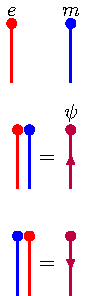
\includegraphics[scale=1]{kinds_of_particles.pdf}
    \end{column}
    \end{columns}
\end{frame}

\begin{frame}
    \frametitle{Rules of the braid, and how particles fuse}
    \begin{columns}
        \begin{column}{0.6\textwidth}
            \begin{itemize}
                \item The electric charge, $e$ is a boson. 
                \item The magnetic vortex, $m$ is a boson. 
                \item $e$ going around $m$ gives a $-1$. 
                \item $\psi$ is a fermion.
                \item The braid group is Abelian. 
            \end{itemize}
        \end{column}
        \begin{column}{0.4\textwidth}
            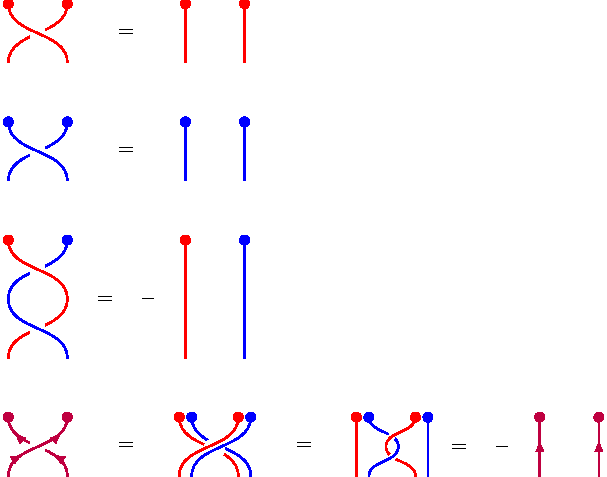
\includegraphics[scale=0.9, trim=0 60 170 0, clip]{rules_of_braiding.pdf}
        \end{column}
    \end{columns}
    \vspace{10pt}
    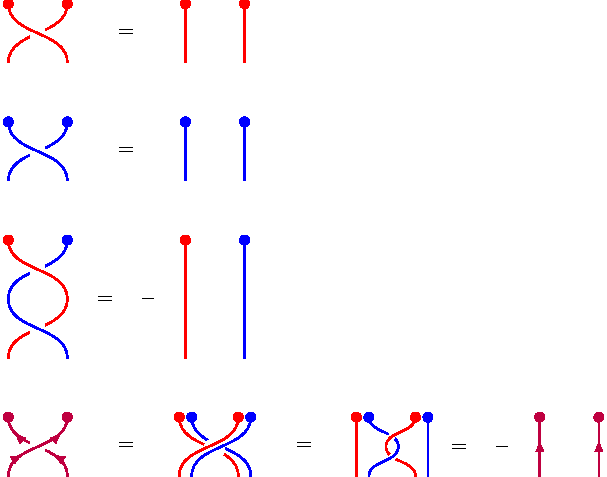
\includegraphics[scale=1, trim=0 0 0 190, clip]{rules_of_braiding.pdf}
\end{frame}

\begin{frame}
    \frametitle{Anyons front and center}
    \framesubtitle{Anyons implies the ground state degeneracy.}

    \begin{framed}
        We want to think of the how the anyons braid, as defining the topological order in the system.
    \end{framed}
    \begin{itemize}
        % \item Let $Z_{i}\ (X_{i})$ be the operation that create an $m\ (e)$ particle pair, take one of them around one of the non-contractible loops of the torus, and annihilate the pair again. 
        \item The ground state(s) is a sate with no particles in it. If $\ket{\Omega_0}$ is a ground state so it $Z_i \ket{\Omega_0}$ and $X_i \ket{\Omega_0}$.
    \end{itemize}
    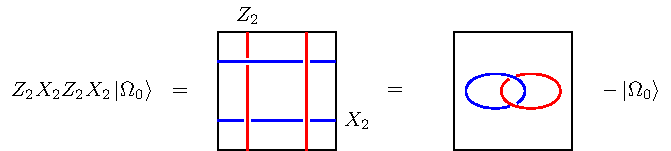
\includegraphics[scale=0.9]{anyons_ground_state.pdf}
    \begin{itemize}
        \item Braiding rules implies \begin{enumerate}
            \item $Z_i^2 = X_i^2 = 1$
            \item $\[Z_1, Z_2 \] = \[X_1, X_2 \] = \[X_1, Z_2 \] = \[Z_1, X_2 \] = 0$
            \item $\{Z_1, X_1 \} = \{Z_2, X_2 \} = 0$.
        \end{enumerate}
        \item This implies the ground state is fourfold degenerate. 
    \end{itemize}
    
    
\end{frame}

\begin{frame}
    \frametitle{Summary}

    \begin{itemize}
        \item Quantum codes encode $k$ qubits into $n$ qubits. 
        \item Quantum codes allow for error correction 
        \item The Kitaev toric code encode $2g$ qubits into a spin lattice.  
        \item The Kitaev code has $e^{-\alpha N}$ probability of missing errors. 
        \item By moving anyons around, one can perform quantum operations on the qubits. 
        \item The anyon content of a theory is enough to define its topological order.
    \end{itemize}

\end{frame}


\bibliographystyle{plainnat}
\bibliography{reference}
\end{document} 
 
